% Put into the format for a VUW thesis chapter Friday 28 March 2014
% Radical rewriting began Monday 31 March 2014

\documentclass[12pt, a4paper, twoside, openright]{book}

\usepackage{vuwthesis} % sets up some local things, mostly the front page

\setlength{\intextsep}{12pt} % set space above and below in-line float
\setlength{\abovecaptionskip}{0pt} % set space between figure and caption.


\usepackage{amssymb, amsmath}
\usepackage{tikz}
\usetikzlibrary{calc}

%\usepackage{marvosym}

\newcommand{\beff}{\ensuremath{b_{\mathrm{eff}}}}
\newcommand{\bhigh}{\ensuremath{b_{\mathrm{high}}}}
\newcommand{\blow}{\ensuremath{b_{\mathrm{low}}}}
\newcommand{\phislip}{\ensuremath{\phi_{\mathrm{slip}}}}
\newcommand{\phisol}{\ensuremath{\phi_{\mathrm{solid}}}}
\newcommand{\sigsol}{\ensuremath{\sigma_{\mathrm{solid}}}}
\newcommand{\gamsol}{\ensuremath{ \dot{\gamma}_{\mathrm{solid}} }} 

\newcommand{\sep}{\begin{equation*} \star \end{equation*}}

\newcommand{\paper}[1]
         {\colorbox[gray]{0.8}{ \textsc{#1}}
         
         }

\usepackage{etoolbox}
\newtoggle{compilealone}
\toggletrue{compilealone}

\title{Chapter 3: Mixed Slip Flow}
\author{Nat Lund}

\begin{document}
\chapter{Mixed-Slip Flow}\label{C:mixedslip}

In this short chapter we look at the challenge of defining a slip length of a surface that is \emph{rough.}   There is some choice as the location of the $z=0$ plane, leading to some ambiguity regarding slip lengths.  The issue is clarified with the concept of the no-slip plane.    We then define two rough surfaces of mixed slip length: superhydrophobic surfaces and surfaces covered with nanobubbles.  Experimental results showing high slip over these surfaces are discussed.  Finally, the concepts in this chapter are illustrated in a description of an experiment in which the presence of nanobubbles appears to \emph{reduce} slip.

\clearpage
\section{Rough Surfaces}

While the slip length of a perfectly flat surface is an intuitive concept, the definition of the slip length of a \emph{rough} surface is more troublesome.  The question ``What is the slip length of this surface?" suddenly acquires a resonance with the old Vaudeville joke ``How's your wife?";  the answer: ``Compared to what?".


\subsection{Rough No-Slip Surfaces}

To clarify, consider Couette-like flow over a rough surface composed of material with \emph{no} intrinsic slip length.  The system \emph{behaves like} an equivalent system with a \emph{flat} no-slip boundary surface.  Define this boundary as the \textbf{effective no-slip plane.}  Where is the position of the effective no-slip plane in relation to the original rough surface?  It is likely to be located at a  level between the troughs and peaks of the roughness, but if the roughness caused significant turbulence, then it may be located \emph{above} the peaks of the roughness.  See Figure (\ref{effnoslipplane}).

\begin{figure}[ht]
\centering
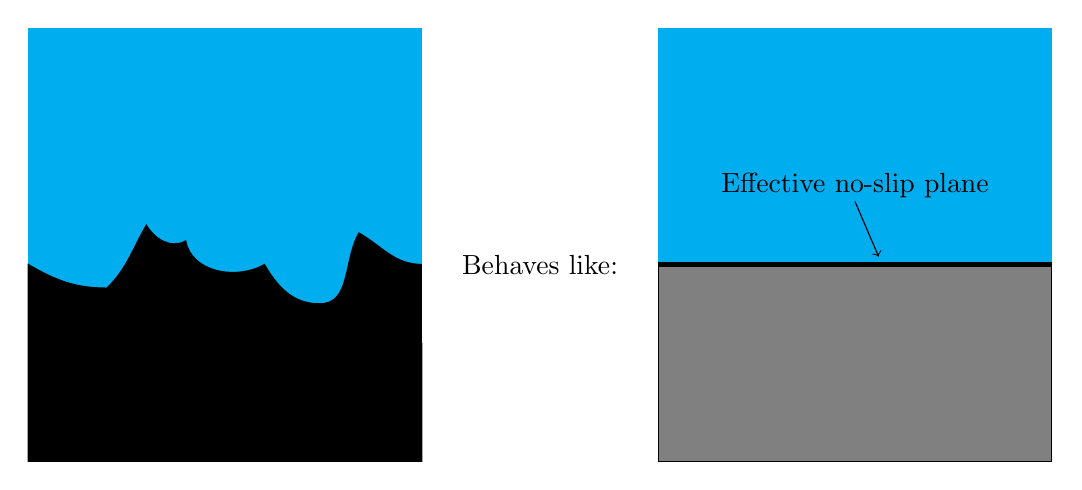
\begin{tikzpicture}

\draw[cyan, fill=cyan] (0,0) rectangle (5,4);

\filldraw (5,0) -- (5,-1.5) -- (0,-1.5) -- (0,1)  to [out=-30,in=180] 
          (1,0.7) to [out=45,in=240] (1.5,1.5)  to [out=-60,in=210] (2,1.3)
           to [out=-80,in=210] (3, 1)  to [out=-60,in=180] (3.7,0.5)
            to [out=0,in=240] (4.2,1.4)  to [out=-30,in=180] (5,1);
            
            
\draw[cyan, fill=cyan] (8,0) rectangle ++(5,4);
\draw[fill=gray] (8,-1.5) rectangle ++(5,2.5);

\draw[ultra thick] (8,1) -- ++(5,0);

%\renewcommand{\baselinestretch}{1.00}
\node at (6.5,1){Behaves like:};
\node at (10.5,2) {Effective no-slip plane};
\draw[->] (10.5,1.8) -- ++(0.3,-0.7);

\end{tikzpicture}
\caption{A rough no-slip surface behaves as if an effective no-slip plane was located somewhere above the troughs of the roughness.}\label{effnoslipplane}
\end{figure}

In a sense, the position of the effective no-slip plane is what is measured by a macro-scale slip experiment. For example: a rough-walled capillary of nominal diameter $d$ flows as much as a smooth-walled capillary of diameter $d_{\mathrm{eff}}$.  Then, loosely speaking, the slip length is the distance between the effective no-slip plane and the physical surface.  But if rough, the physical surface is not a plane, but a nominal surface \emph{region} of finite width.  The issue then, is to decide where to locate a flat \emph{reference plane}, from which to measure the slip length.  The reference plane corresponds to the $z=0$ plane in the mathematical model of the system.  See Figure (\ref{referenceplane}).

\begin{figure}[ht]
\centering
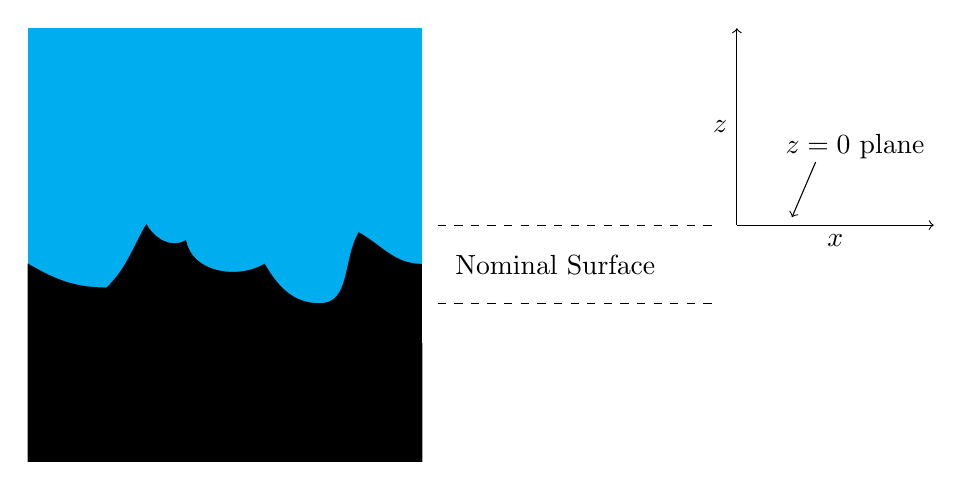
\begin{tikzpicture}

\draw[cyan, fill=cyan] (0,0) rectangle (5,4);

\filldraw (5,0) -- (5,-1.5) -- (0,-1.5) -- (0,1)  to [out=-30,in=180] 
          (1,0.7) to [out=45,in=240] (1.5,1.5)  to [out=-60,in=210] (2,1.3)
           to [out=-80,in=210] (3, 1)  to [out=-60,in=180] (3.7,0.5)
            to [out=0,in=240] (4.2,1.4)  to [out=-30,in=180] (5,1);
       
\draw[dashed] (5.2,0.5) -- +(3.5,0);
\draw[dashed] (5.2,1.5) -- +(3.5,0);

\node at (5.3,1)[right]{Nominal Surface};

\draw[->] (9,1.5) -- node[left]{$z$} ++(0,2.5);
\draw[->] (9,1.5) -- node[below]{$x$} ++(2.5,0);
     

\node at (10.5,2.5) {$z=0$ plane};
\draw[->] (10,2.3) -- ++(-0.3,-0.7);

\end{tikzpicture}
\caption{The $z=0$ plane of the mathematical model maps to some part of the nominal surface region of the physical surface.}\label{referenceplane}
\end{figure}

Once the location of the $z=0$ plane has been chosen, a slip length can be defined as the distance between the $z=0$ plane and the effective no-slip plane.  By convention, if the effective no-slip plane is \emph{below} the $z=0$ plane, then $b$ is positive.  Obviously, if the $z=0$ plane is located at the bottom of the troughs of the roughness, then the slip length could be \emph{negative.}  See Figure (\ref{roughsliplengths}).

\clearpage
\begin{figure}[ht]
\centering
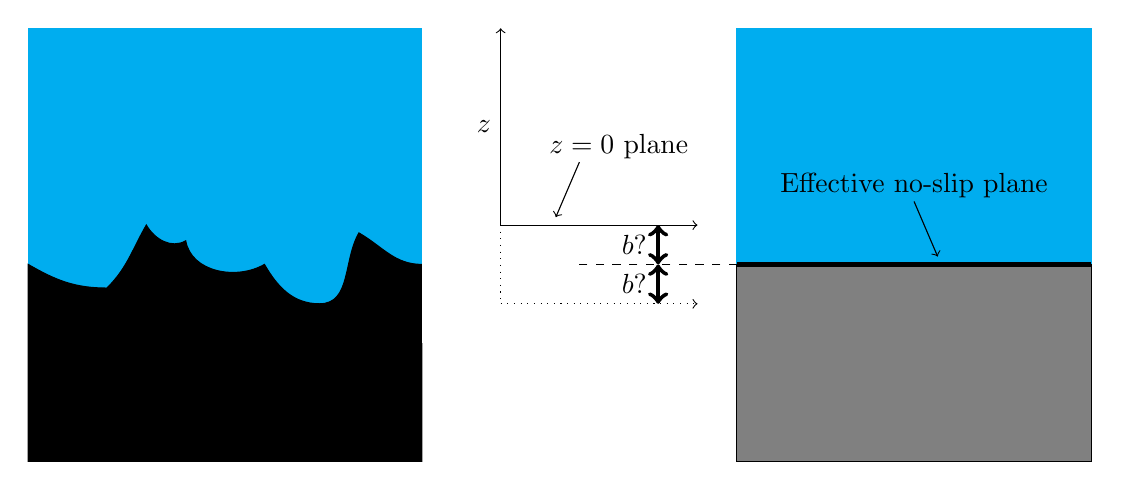
\begin{tikzpicture}

\draw[cyan, fill=cyan] (0,0) rectangle (5,4);

\filldraw (5,0) -- (5,-1.5) -- (0,-1.5) -- (0,1)  to [out=-30,in=180] 
          (1,0.7) to [out=45,in=240] (1.5,1.5)  to [out=-60,in=210] (2,1.3)
           to [out=-80,in=210] (3, 1)  to [out=-60,in=180] (3.7,0.5)
            to [out=0,in=240] (4.2,1.4)  to [out=-30,in=180] (5,1);
            

\draw[->] (6,1.5) -- node[left]{$z$} ++(0,2.5);
\draw[->] (6,1.5) -- ++(2.5,0);% node[below]{$x$} ++(2.5,0);
\draw[dotted] (6,1.5) -- ++(0,-1);
\draw[dotted,->] (6,0.5) -- ++(2.5,0);% node[below]{$x$} ++(2.5,0);     

\node at (7.5,2.5) {$z=0$ plane};
\draw[->] (7,2.3) -- ++(-0.3,-0.7);


\draw[cyan, fill=cyan] (9,0) rectangle ++(4.5,4);
\draw[fill=gray] (9,-1.5) rectangle ++(4.5,2.5);

\draw[ultra thick] (9,1) -- ++(4.5,0);

\node at (11.25,2) {Effective no-slip plane};
\draw[->] (11.25,1.8) -- ++(0.3,-0.7);



\draw[dashed] (9,1) -- ++(-2,0);
\draw[<->,ultra thick] (8,1) -- node[left]{$b$?} ++(0,0.5);
\draw[<->,ultra thick] (8,1) -- node[left]{$b$?} ++(0,-0.5);

\end{tikzpicture}
\caption{The measured slip length of a rough surface depends on the choice of location of the $z=0$ plane.}\label{roughsliplengths}
\end{figure}


The importance of defining the location of the $z=0$ plane was first made explicit in a paper by Vinogradova and Yakubov in 2006 \cite{VinogradovaYakubov2006}.
They used a purpose-built AFM device that tapped a roughened sphere onto a smooth plane.  The sphere had an rms roughness of 10 - 11 nm, and a maximum peak-to-valley distance of 45 nm.  With the surface taken to be at the tops of the peaks, a reduction in drainage force was observed, compared to a smooth sphere of equal diameter.  But the reduction was not due to slip:  The force was equivalent to that of a smooth sphere whose surface was located at an intermediate position between the peaks and valleys of the roughness.

Thus the issue is clarified: if the boundary is taken to be at the valleys of the roughness, then roughness reduces slip.  Conversely, if the boundary is taken to be at the tops of the peaks, then roughness \emph{increases} slip.
They note ``We believe our paper entirely clarifies the situation with flow past rough surfaces, highlights reasons for existing controversies, and resolves apparent paradoxes."

The phrase `effective no slip plane'  first appears in an article by
Kunert and Harting in 2007 \cite{KunertHarting2007}.
%Kunert and Harting in 2007 \cite{KunertHarting2007} formalized the concept with the introduction of an `effective no slip plane', typically located between the peaks and valleys of the surface roughness.  
They carried out numerical simulations using lattice Boltzmann methods on different surfaces.  Each surface has minimum and maximum heights, $h_{\mathrm{min}}$ and $h_{\mathrm{max}}$, and an average height $h_{\mathrm{average}}$.  They calculate the position of the effective no-slip plane, $h_{\mathrm{eff}}$.  In all cases, $h_{\mathrm{eff}}$ was always considerably higher than $h_{\mathrm{average}}$.  If the surface has a few very tall but sparsely distributed spikes, then $h_{\mathrm{average}}$ can be much smaller than $h_{\mathrm{max}}$, and $h_{\mathrm{eff}}$ lies somewhere between them and cannot be well approximated by either.

\vspace*{1em}

The ``existing controversies" and ``apparent paradoxes" mentioned by Vinogradova and Yakubov in \cite{VinogradovaYakubov2006} include a 2002 paper by Zhu and Granick \cite{ZhuGranick2002} showing that roughness suppresses slip, and a 2003 paper by Bonaccurso, Butt and Craig \cite{BonaccursoButtCraig2003} claiming that roughness could increase slip, even on a hydrophilic surface:

%%%%%%%%%%%%%%%%%%%%%%%%%%%%%%%%%%%%%%%%%%%%%%%%%%%%%%

In 2002, Zhu and Granick published results of drainage force experiments on hydrophobic surfaces of varying roughness \cite{ZhuGranick2002}.  The molecularly smooth surface showed a flow dependent slip length of up to 35 nm, while rougness \emph{suppressed} slip, with a roughness of 6 nm giving no slip at all.
They defined the $z=0$ level in the surface force appartatus by `adhesive contact in air'.  Therefore, the $z=0$ level could well be below the tops of the roughness peaks.  No effort was made to account for this.


The paper from 2003 by Bonaccurso, Butt and Craig \cite{BonaccursoButtCraig2003} claimed that roughness could \emph{increase} slip, even on a \emph{hydrophilic} (contact angle zero!) surface.
They measure drainage forces of a glass sphere approaching a silicon surface roughened up to 12.2 nm rms.
They discuss the importance of defining the zero distance.  They end up defining it at the tops of the peaks, as this is the first point of contact.  They calculate slip lengths by fitting the data to Vinogradova's model.  The best fit is when they fix the slip length on the glass sphere at about 43 nm, and increase the slip length of the substrate as roughness increases.  Under `normal' conditions, they find a slip length of 3.5 nm for maximum roughness of 12.2 nm.  But for extremely high approach velocities, for the same roughness they find a slip length of 900 nm!


\clearpage
\subsubsection{ Surfaces with Slip}

If a rough surface has a non-zero intrinsic slip length on all or part of its surface,  then the effective no-slip plane may be located well below the nominal surface region.  There will still be a range of reasonable effective slip lengths, depending on the choice of the location of the $z=0$ plane.  See Figure (\ref{roughslip}).  

\begin{figure}[ht]
\centering
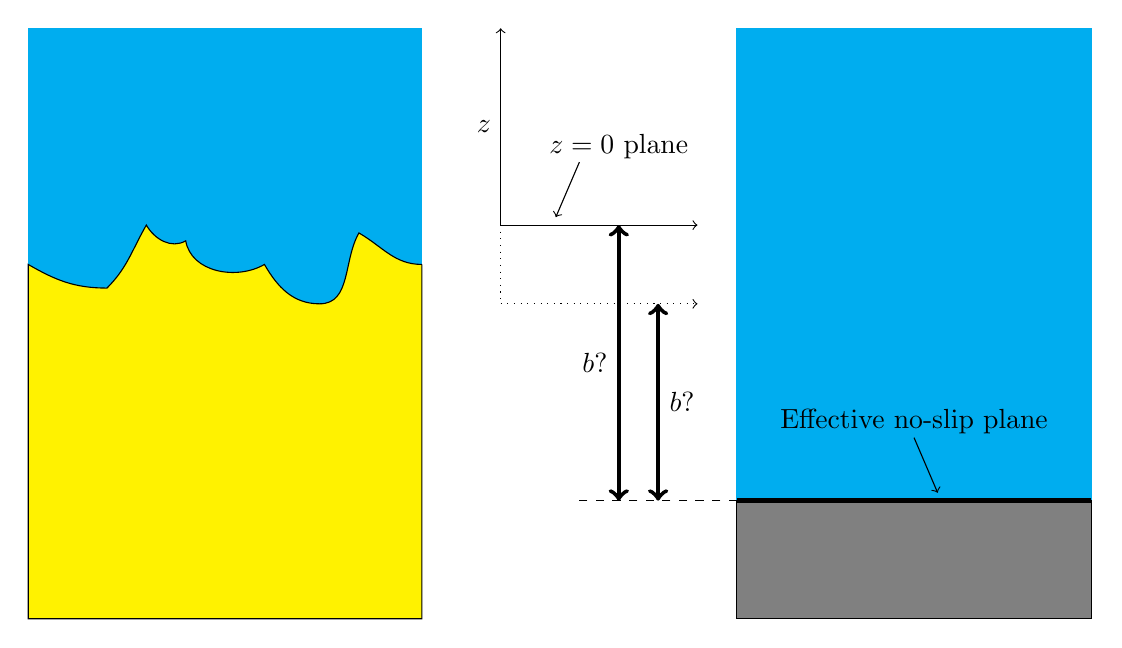
\begin{tikzpicture}

\draw[cyan, fill=cyan] (0,0) rectangle (5,4);

\draw[fill=yellow] (5,1) -- (5,-3.5) -- (0,-3.5) -- (0,1)  to [out=-30,in=180] 
          (1,0.7) to [out=45,in=240] (1.5,1.5)  to [out=-60,in=210] (2,1.3)
           to [out=-80,in=210] (3, 1)  to [out=-60,in=180] (3.7,0.5)
            to [out=0,in=240] (4.2,1.4)  to [out=-30,in=180] (5,1);
            

\draw[->] (6,1.5) -- node[left]{$z$} ++(0,2.5);
\draw[->] (6,1.5) -- ++(2.5,0);% node[below]{$x$} ++(2.5,0);
\draw[dotted] (6,1.5) -- ++(0,-1);
\draw[dotted,->] (6,0.5) -- ++(2.5,0);% node[below]{$x$} ++(2.5,0);     

\node at (7.5,2.5) {$z=0$ plane};
\draw[->] (7,2.3) -- ++(-0.3,-0.7);


\draw[cyan, fill=cyan] (9,-2) rectangle ++(4.5,6);
\draw[fill=gray] (9,-3.5) rectangle ++(4.5,1.5);

\draw[ultra thick] (9,-2) -- ++(4.5,0);

\node at (11.25,-1) {Effective no-slip plane};
\draw[->] (11.25,-1.2) -- ++(0.3,-0.7);



\draw[dashed] (9,-2) -- ++(-2,0);
\draw[<->,ultra thick] (8,-2) -- node[right]{$b$?} ++(0,2.5);
\draw[<->,ultra thick] (7.5,-2) -- node[left]{$b$?} ++(0,3.5);

\end{tikzpicture}
\caption{The measured slip length of a rough surface with intrinsic slip depends on the choice of the location of the $z=0$ plane.}\label{roughslip}
\end{figure}

Note that it is still possible to get a \emph{negative} slip length on a surface with high intrinsic slip lengths, if the $z=0$ plane is located at the bottom of the valleys of the roughness.  In general, the best choice for the location of the $z=0$ plane is at the \emph{tops of the peaks} of the roughness, ensuring that slip lengths are usually positive. 

\clearpage
\section{Mixed-Slip Surfaces}

We turn now to study surfaces in which the intrinsic slip length varies over the surface.
Dramatic variations in the intrinsic slip length of a surface may be achieved if part of the surface is composed of gas.  The intrinsic slip length of the liquid-gas interface is expected to be large compared to that of the liquid-solid interface.  There are two solid-gas surface types important to current research: superhydrophobic surfaces and surfaces with nanobubbles.
Because the liquid-gas interface is a \emph{meniscus} that is usually curved, by their nature, these surfaces are usually rough.  (Having said that, they are sometimes modelled as being flat.)

\subsection{Superhydrophobic Surfaces}

Recall that when a droplet of water sits on a surface, a contact angle $\theta$ is defined as in Figure (\ref{contactangle}).

\begin{figure}[ht]
\centering
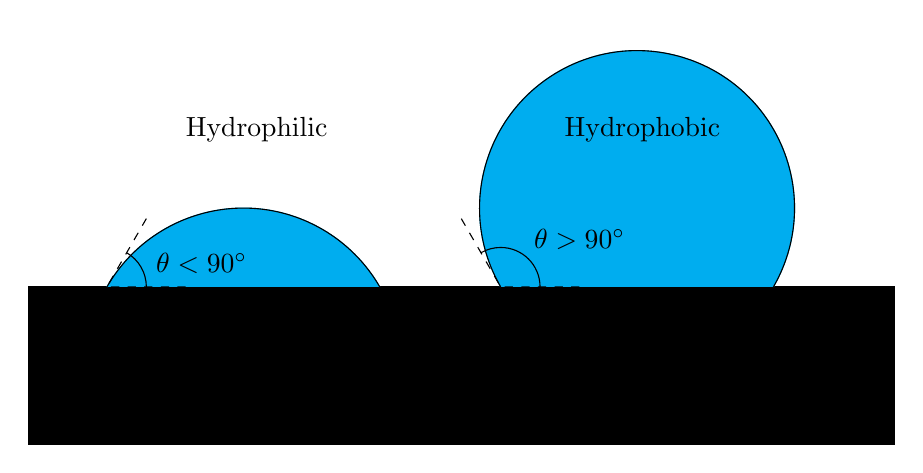
\begin{tikzpicture}
\filldraw (-1,0) rectangle +(11,-2); 

\filldraw[color=cyan] (0,0) arc (150:30:2);
\draw (0,0) arc (150:30:2);

\draw[dashed] (1,0) -- (0,0) -- (0.5,0.866);
\draw (0.5,0) arc (0:60:0.5);
\node at (0.5,0.3)[right] {$\theta < 90^{\circ}$};

\filldraw[color=cyan] (5,0) arc (210:-30:2);
\draw (5,0) arc (210:-30:2);

\draw[dashed] (6,0) -- (5,0) -- +(-0.5,0.866);
\draw (5.5,0) arc (0:120:0.5);
\node at (5.3,0.6)[right] {$\theta > 90^{\circ}$};

\node at (1.9,2) {Hydrophilic};
\node at (6.8,2) {Hydrophobic};

\end{tikzpicture}
\caption{The contact angle $\theta$ of a surface.}\label{contactangle}
\end{figure}

Usually, a surface is defined as \emph{hydrophobic} when the contact angle is more than $90^{\circ}$.
%This means that the water molecules are more attracted to each other than they are to the surface. 
(If $\theta < 90^{\circ}$, the surface is \emph{hydrophilic}.  If $\theta \sim 0^{\circ}$, then \emph{complete wetting} occurs: the water spreads out as far as it can.)

Tiny, micron or nanometer scale pillars can be constructed out of hydrophobic material.  A collection of theses hydrophobic nanopillars can be affixed to a suitable substrate, forming a `nanoforest'.  (Or, more practically, a nanoforest can be constructed, then chemically treated to become hydrophobic.)  If a water droplet is placed on top of the nanoforest, two curious things happen:  First, the droplet sits on the tops of the nanopillars, supported by surface tension.  Second, the apparent contact angle is very large, well over 90$^{\circ}$.  An illustration appears in Figure (\ref{superhydrophobic}).  Due to the extremely high contact angle, these nano or micro-structured surfaces are known as \emph{superhydrophobic} surfaces.  

\begin{figure}[ht]
\centering
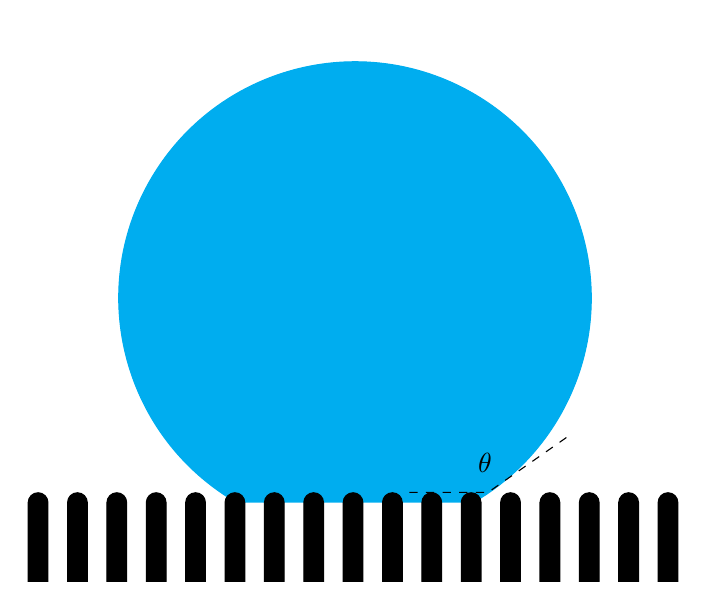
\begin{tikzpicture}

\filldraw[color=cyan] (3.15,1) arc (240:-60:3);

\foreach \x in {1,2,...,17}
{ \filldraw (\x/2,0) rectangle +(0.25,1) arc (0:180:0.125); }

\draw [dashed] (5.34,1.13) -- ++(1,0) -- ++(1,0.7);
\node at (6.3,1.5) {$\theta $};

\end{tikzpicture}
\caption{Superhydrophobicity: surface tension supports a water drop on top of nanopillars, with a very high apparent contact angle}\label{superhydrophobic}
\end{figure}

  

%This second effect is caused by the fact that at the point where the contact line is located, the solid surface is at an angle to the plane of the nanoforest.

%\begin{figure}
%\centering
%\begin{tikzpicture}
%
%\filldraw[color=cyan] (10.5,6) -- (-1,6) -- (-1,2) arc (270:300:2.5)  -- +(1.5,0) arc (240:300:2.5) -- 
%(5.75,2.54)  arc (-80:-64:18);
%
%\foreach \x in {0,1,2}
%\filldraw (\x*4,0) rectangle +(2,2) arc (0:180:1);
%
%\draw[dashed] (5.85,2.55) -- +(-0.5,0.7);
%\draw[dashed] (5.85,2.55) -- +(0.8,0.15);
%\node at (6,2.9) {$\theta$};
%
%\draw[very thick, dashed] (10, 3) -- +(-3,0);
%\draw[very thick, dashed] (7.7,3) -- +(2,0.6);
%\draw[very thick] (7.2,3) arc (180:20:0.5);
%\node at (7.7,4) {Apparent $\theta$};
%
%\end{tikzpicture}
%\caption{c}\label{c}
%\end{figure}


Such surfaces were constructed as early as 1996.  Onda \emph{et al} \cite{Onda1996} discussed the theoretical contact angle of such a surface, and demonstrated a ``super-water-repellent fractal surface'' made of alkylketene dimer, with a remarkable contact angle of $174^{\circ}$.

Enormous contact angles are routinely quoted for static droplets.  The contact angle is slightly different if the droplet is advancing (or retreating).  This hysteresis was studied, for example, by Kusumaatmaja and Yeomans in 2007 \cite{KusumaatmajaYeomans2007}.

\clearpage
But perhaps more interestingly, superhydrophobic surfaces were first observed in nature. The sacred lotus is an aquatic plant (not a water lily, but similar) whose water-repellent qualities have been noted since antiquity.  A passage in the Baghavad Gita states ``One who performs his duty without attachment, ... is unaffected by sinful action, as the lotus is unaffected by water."
In 1993, Barthlott and Neinhuis were taking scanning electron micrographs of the leaf surfaces of some 10,000 plant species.  They noticed that \emph{flat} surfaces always had to be cleaned before examination, while certain rough waxy surfaces did not.  They characterised these self-cleaning surfaces as covered with wax crystalloids ``in a regular microrelief of about 1 - 5 $\mu$m" -- i.e. superhydrophobic.  They describe the cleaning mechanism: Water beads into near-spherical droplets, which easily roll off the leaf.  Dirt particles tend to be hydrophilic, and only weakly bound to the tops of the roughness.  Thus the dirt particles are captured by the water droplets, and move with them off the leaf.  More from antiquity: a Confucian scholar wrote ``I love the lotus, because while growing in mud, it is unstained." In a pair of papers in 1997 \cite{BarthlottNeinhuis1997,NeinhuisBarthlott1997}, Barthlott and Neinhuis describe their studies of what they dub the `lotus effect'.

The image of a droplet supported by thin spikes inspires another metaphor: a Fakir (malnourished Yoga practitioner) sitting on a bed of nails.  David Qu\'{e}r\'{e}'s article `Fakir droplets' gives a very readable summary of the state of affairs in 2002 \cite{Quere2002}.  The quote of relevance to this thesis is the last few sentences of the article: ``On a superhydrophobic solid, however, drops seem to move over a dynamic film of air --- which makes the friction comparable to that experienced by a raindrop falling in air.  But what happens if these textured solids are fully immersed in a pool of water? Will the water still slide on them?  Except for a few controversial studies, this question still remains open, and designers of boats and swimsuits impatiently await an answer."

These questions form the backdrop to the line of research leading to this thesis.

\subsection{Nanobubbles}

In 2001, Tyrrell and Attard discovered what appeared to be nanobubbles on hydrophobic surfaces \cite{TyrrellAttard2001}.   An extract from the abstract of their paper in Physical Review Letters says it all: ``Imaging of hydrophobic surfaces in water with tapping mode atomic force microscopy reveals them to be covered with soft domains, apparently nanobubbles, that are close packed and irregular in cross section, have a radius of curvature of the order of 100 nm, and a height above the substrate of 20 -- 30 nm."  
See schematic of Figure (\ref{nanobubbles}).

It had been observed that when two hydrophobic bodies were brought together underwater, at some very close separation, a `hydrophobic force' suddenly pulled them together.  In 2002, Tyrrell and Attard published \cite{TyrrellAttard2002} more AFM images of nanobubbles, and proposed them to be the origin of the `hydrophobic force'.

\begin{figure}[ht]
\centering
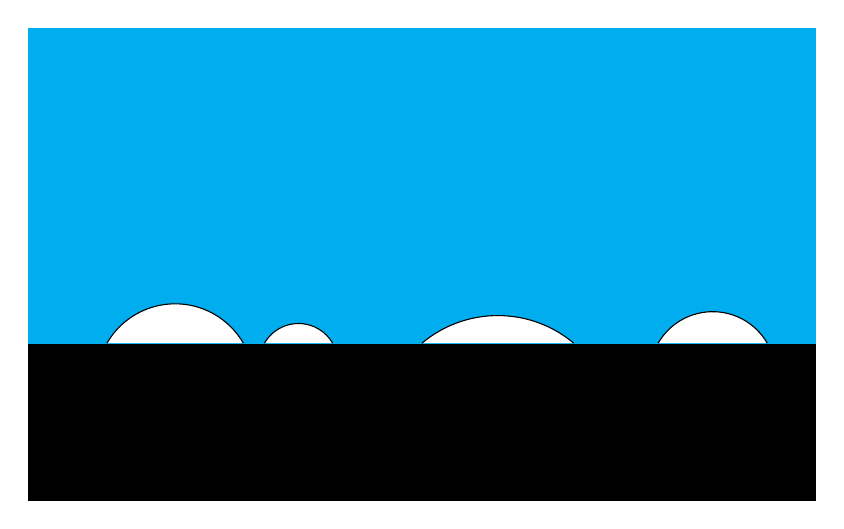
\begin{tikzpicture}
\filldraw (0,0) rectangle (10,-2);
\filldraw[color=cyan] (0,0) rectangle (10,4);

\draw[fill=white] (1,0) arc (150:30:1);
\draw[fill=white] (3,0) arc (150:30:0.5);
\draw[fill=white] (5,0) arc (130:50:1.5);
\draw[fill=white] (8,0) arc (150:30:0.8);

\end{tikzpicture}
\caption{Nanobubbles of gas on a solid surface.}\label{nanobubbles}
\end{figure}

The question naturally arises: when are nanobubbles present?  Yang and coworkers published in 2007 \cite{Yang2007} an exhaustive experimental study on the factors influencing the formation of nanobubbles, such as temperature, dissolved gases etc.  It turns out that if a surface had been immersed in ethanol before being immersed in water, then nanobubbles are reliably formed.  

Using this `solvent exchange' technique, Zhang, Quinn and Ducker in 2008 \cite{ZhangQuinnDucker2007} were able to do repeatable studies of nanobubbles.  Using infrared spectroscopy, they confirmed the presence of a gas phase 5 -- 80 nm thick at the surface --- i.e. good evidence that the `soft domains' really are nanobubbles.
An AFM was used to determine the radius of curvature of the bubbles; the implied Laplace pressure in the bubbles was found to be 1.0 -- 1.7 atmospheres.  This pressure allows nanobubbles of air to remain stable for days.  They find that nanobubbles form much more easily on rough surfaces, sometimes even without the solvent exchange technique.

%Crucially, the solvent exchange technique is also a common cleaning technique.  Therefore, nanobubbles may be formed inadvertently in the process of a slip experiment.  

Given the fact that rough surfaces may spontaneously form nanobubbles, the question arises:  How many ostensibly `pure' slip experiments are actually experiments on \emph{mixed-slip} surfaces?
A purpose of the research in this thesis is to give some indication of the effect of such nanobubble contamination on a slip experiment.

\vspace*{1em}
In summary, mixed-slip surfaces tend to fall into the two types described above: either a solid surface interspersed with pockets of air (nanobubble type), or a gas-liquid interface interspersed with islands of solid material (superhydrophobic type).  Thus, a superhydrophobic type surface has a contiguous \emph{air-liquid} interface, while a nanobubble type surface has a contiguous \emph{solid} phase.

In the two-dimensional case, the difference disappears.  \emph{Neither} the solid-liquid nor air-liquid interfaces are contiguous.  Physically, this surface consists of a grating of parallel ridges, with an air gap between the ridges.  The liquid sits on the top of the ridges, and the air-liquid interface forms a meniscus between the ridges.

\clearpage
\section{Rough Mixed-Slip Flow}

\subsection{High Slip Over Solid-Gas Surfaces}


In 2003, Cottin-Bizonne \emph{et al} published a paper \cite{Cottin-Bizonne2003} in which they stated ``Our results show for the first time that, in contrast to common belief, surface friction may be reduced by surface roughness."  In fact, what they discovered is that flow over a rough surface may transition into the superhydrophobic state, with the fluid now flowing over vapour pockets.  
%(As previously stated, later that same year, Bonaccurso, Butt and Craig \cite{BonaccursoButtCraig2003} experimentally demonstrated that roughness increases slip. But they did not explicitly consider that their system may have entered the superhydrophobic regime.  Had it?)

Cottin-Bizonne and coworkers looked at molecular dynamics simulations of a Lennard-Jones fluid flowing over a flat surface decorated with narrow square posts.  At sufficiently low pressures, the fluid entered the Cassie state, as a vapour phase spontaneously formed at the surface, leaving the fluid supported on top of the posts.  The surface had an intrinsic slip length of 20 - 25 $\sigma$ (atom diameters).  In the Cassie state, effective slip lengths up to 57 $\sigma$ appeared.  For very narrow posts -- 4.9 $\sigma$, slip lengths could reach 130 $\sigma$.  Note that slip lengths were measured from the bottom of the cavity, so the post height --- 6 $\sigma$ --- could be added to the slip lengths.

\vspace{1em}
A physical demonstration of this superhydrophobic Cassie state flow was presented by Choi and Kim in 2006 \cite{ChoiKim2006}.  They were probably the first to deliberately engineer a surface for maximum slip: `nanoturf', silicon nanoposts about 1 - 2 $\mu$m high, spaced about 0.5 - 1.0 $\mu$m apart, rendered hydrophobic by a 10 - 20 nm thick layer of Teflon.  They estimated the air fraction of the surface to be 60 \%.

A commercial cone-and-plate rheometer was used to measure slip lengths: a collosal 20 $\mu$m for water and 50 $\mu$m for 30 \% glycerine solution.  (They expect this, since the viscosity of the glycerine solution is 2.5 times greater than that of water.)

\vspace*{1em}
Such high slip lengths were not replicated in a more careful study by Joseph \emph{et al} also in 2006 \cite{Joseph2006}.  They did particle image velocimetry on channels coated with carbon nanotubes of diameter 50 - 100 nm, spaced 100 - 250 nm apart.  The tops of the nanotubes could be evenly spaced, or clumped together like wet hair, giving inter-clump length scales of 1.7, 3.5 or 6 $\mu$m.  The derived slip lengths for the three surface morphologies were roughly 0.4, 1.0 and 1.4 $\mu$m, respectively.

They note that their results are an order of magnitude smaller than the 20 $\mu$m slip lengths of Choi and Kim, and point out that rheological methods lack the sensitivity to measure surface effects.

An effort was made by Lee and Kim in 2011 \cite{LeeKim2011} to maximize slip by making a heirarchical structured surface --- nanoposts on top of microposts.  It worked if area fraction taken up by the microposts was large enough.  Below about 10\% area fraction --- a realistic figure --- the advantage began to disappear, and at 4\% area fraction, the heirarchical surface gave \emph{lower} slip than conventional unadorned microposts.

\vspace*{1em}

A one-dimensional version of the superhydrophobic surface is a nanograting --- a surface covered with ridges, with the water supported by surface tension on top of the ridges.  In 2006, Choi \emph{et al} \cite{Choi2006} presented slip experiments on a ``well-defined nanograte": ridges 500 nm high and 50 nm wide, separated by a gap of 180 nm.  Thus the pitch (period) was 230 nm.
If the grating was left hydrophilic, they believe that water fully wets the surface, penetrating down into the troughs.  After rendering the surface hydrophobic with Teflon, they believe that there is air in the troughs.  Experiments were carried out with both states, with fluid flow both parallel to, and transverse to the ridges.

They could measure slip lengths to a resolution of only 30 nm, thus they were unsure if the hydrophobic surface had any intrinsic slip.  For flow parallel to the ridges, there was a clear distinction between the slip lengths of hydrophilic and hydrophobic surfaces.  $30 \pm 15$ nm for hydrophilic, and $143 \pm 35$ nm for hydrophobic.  For transverse flow, they found insignificant slip, $0 \pm 17$ nm for hydrophilic, and $61 \pm 44$ nm for hydrophobic.



\subsubsection{Protruding Nanobubbles Reduce Slip}

As noted earlier, roughness may apparently decrease the effective slip length, if the reference $z=0$ plane is taken to be at the lowest point of the roughness.  This was an appropriate choice for the experimental setup of Steinberger \emph{et al} of 2007 \cite{Steinberger2007}.

One can imagine the difficulties in studying a surface of nanobubbles, given their random, uncontrolled nature.  Steinberger \emph{et al} addressed the issue by studying flow over a flat surface covered with holes 1.3 $\mu$m wide and 3.5 $\mu$m deep.  Air can be trapped in the holes; they derive slip lengths via drainage force measurements on the resulting microbubble surface.

The plane $z=0$ is located on the flat surface, at the tops of the holes.  In the Wenzel state, with water filling the holes, they measure a slip length of $105 \pm 10$ nm.  With air trapped in the holes they find a \emph{lower} slip length: a mere $20 \pm 10$ nm.
%  Understandably, they are puzzled by this, so they investigate.  
They discover that the microbubbles protrude an estimated 200 - 400 nm above the flat surface, with the meniscus subtending an angle between $30^{\circ}$ and $60^{\circ}$ to the flat surface.  Is this protrusion into the bulk the cause of low slip lengths?

They test this hypothesis numerically, with a finite element package (Comsol).  They find a flat bubble ($\theta = 0^{\circ}$) gives maximum slip length --- about 160 nm.  Any increase in $\theta$ decreased slip, with $\theta > 45^{\circ}$ giving a lower slip length than the Wenzel state.

\vspace*{1em}
The following year (2008) Hyv\"{a}luoma and Harting replicate and extend Steinberger's numerics \cite{HyvaluomaHarting2008}.  By using lattice Boltzmann methods, they can model the bubble deforming under stress.  They essentially replicate Steinberger: a maximum slip of about 150 nm at zero protrusion angle, plummeting down past zero slip length for a protrusion angle greater than about $70^{\circ}$

They simulate Couette flow, so are able to investigate shear dependence.  In steady state shear-driven flow, they see a \emph{decrease} in slip length with increasing shear.  This contradicts some earlier claims.  However, higher shear rates deform the microbubbles, reducing the average height of the microbubbles.


\vspace*{1em}

Incidentally, the idea that slip is reduced by protruding bubbles had been proposed by Lauga and Brenner in 2004 \cite{LaugaBrenner2004}.  In a theoretical paper, they present a model to explain the shear-dependent slip found by Zhu and Granick in 2001 \cite{ZhuGranick2001}.  They assume that the surface was (unknown to the experimenters) covered in bubbles.  Slip lengths were inferred from the drainage force of a probe slamming into the surface at various speeds. As the probe approach velocity increases, so too does the pressure in front of it.  This increased pressure causes the bubbles to shrink, both from compression of the gas and increased diffusion into the liquid.  The reduced bubble height widens the channel, making drainage easier, for a given probe-surface distance.  Thus, this `leaking mattress effect' causes a
\nopagebreak[0] shear-dependent slip effect to appear.


\section{Conclusion}

In summary, high slip lengths are possible over mixed-slip surfaces: more than 100 nanometers for nanogratings, and more than 1 micron for nanoforests.  However, the effective slip length has a slightly ambiguous definition; the quoted slip length depends on the nominal position of the $z=0$ plane.  Things are clarified by introducing the concept of an effective no-slip plane.  This is an objective concept: the surface behaves as if the no-slip plane was located at a given position.  Then, the slip length is the distance between $z=0$ and the effective no-slip plane.  Thus, if the no-slip plane becomes lower, then the slip length is increased, and vice versa.  A sensible choice for the position of the nominal $z=0$ plane is the \emph{top of the roughness.}  That way, quoted slip lengths will often be positive.  Note that if the $z=0$ plane was chosen to be \emph{below} the no-slip plane to start with, lowering the no-slip plane still \emph{increases} the slip length.  Another benefit is that a physical instrument probing the surface will tend to encounter the surface peaks, and record that as the surface position.
% by making it \emph{less negative.}

%\begin{center} \vspace{3em} \Coffeecup \end{center}

\iftoggle{compilealone}
    {
    \bibliography{Lund_Thesis.bib}
    \bibliographystyle{plain}
    }

\end{document}
